\documentclass[../sparc.tex]{subfiles}
\graphicspath{{\subfix{../images/}}}
\begin{document}

%%%%%%%%%%%%%%%%%%%%%%%%%%%%%%%%%%%%%%%%%%%%%%%%%%%%%%%%%%%%%%%%%%%%%%%%%%%%%%%%
\newpage
\section{Musical staff}
\index{Music!Musical staff}

We can program simple melodies without knowing the musical notation.  For
example, we can use complete examples from the internet -- and for most of
popular melodies we can find notes written in scientific notation (or even we
can find complete programs for Arduino that play music!)  But at some point we
can find ourselves in the situation where all we have is just a musical score
and no more.  Because of that, before we go further, we have to get some grasp
on the \emph{musical staff}.

Let's take another look on the melody ``Twinkle, Twinkle, Little Star''.

\begin{figure}[ht]
  \centering
  \begin{lilypond}
    \relative c' {
      \numericTimeSignature
      \time 4/4
      c4 c g' g
      a a g2
      f4 f e e
      d d c2
      g'4 g f f
      e e d2
      g4 g f f
      e e d2
      c4 c g' g
      a a g2
      f4 f e e
      d d c2
    }
    \layout {
      indent = 0\mm
      line-width = 100\mm
      ragged-last = ##t
    }
  \end{lilypond}
  \label{fig:sound-fig-4}
  \caption{``Twinkle, Twinkle, Little Star''}
\end{figure}

Before we ignored the position of notes on the ``Y'' axis and used only the
``already decoded'' notes, written in the scientific notation.  Now it's the
time to look closely on those groups of five lines and the symbols on them.

Let's start from the lines -- they are called the \emph{musical staff}.

\index{Music!Treble clef} The notes and other symbols are written on top of the
staff.  At the beginning of a musical composition a special big ``squiggle'' is
written, which is called \emph{clef}.  The clef allows us to read the notes on
the staff and their octaves.  In the ``Twinkle, Twinkle, Little Star'' melody
(\ref{fig:sound-fig-4}) only one type of clef is used which is called
\emph{treble clef}.  This clef circles the second line from the bottom on the
staff and that means that the line represents ``G4'' note (as is shown on fig.
\ref{fig:lilypond-clef-example}.)

\begin{figure}[ht]
  \centering
  \begin{lilypond}
    \relative c' {
      \numericTimeSignature
      \time 4/4
      g'1
    }
  \end{lilypond}
  \label{fig:lilypond-clef-example}
  \caption{Treble clef and the ``G4'' note.}
\end{figure}

As we can see on the figure above, the second line from the bottom holds the
``G4'' note, as the line is circled by the treble clef.  That means that all
notes written on this line are ``G4'' (the ``G'' note from the fourth octave.)

But notes can be written not only on the lines, but in the middle between lines.

Schematically it can be described as the graph, which is shown on the
fig. \ref{fig:lilypond-music-graph-1}.

\begin{figure}[ht]
  \centering
  \begin{tikzpicture}
    \node (image) at (2, 0) { \resizebox{1.0\textwidth}{!}{
        \begin{lilypond}
          \relative c' {
            \numericTimeSignature
            \time 4/4
            c8 d8 e8 f8 g8 a8 b4
          }
        \end{lilypond}
      }
    };
    \foreach \n [count=\i, evaluate=\i as \y using real(\i / 2.6)] in {
      C4, E4, G4, B4, D5, F5
    } {
      \node at (-3.3, \y - 1.6) {\tiny \n};
    };
    \foreach \n [count=\i, evaluate=\i as \y using real(\i / 2.6)] in {
      D4, F4, A4, C5, E5, G5
    } {
      \node at (-3.0, \y - 1.4) {\tiny \n};
    };
    \draw[thick, ->] (-4.0, -2.0) -- (8.0, -2.0) node[anchor=north east] {x};
    \draw[thick, ->] (-4.0, -2.0) -- (-4.0, 1.5) node[anchor=north east] {y};
  \end{tikzpicture}
  \label{fig:lilypond-music-graph-1}
  \caption{A musical ``graph''.  ``x'' axis represents time, and ``y'' axis
    represents the sound frequency.}
\end{figure}

On this musical graph we can see the notes are arranged in order: ``C'', ``D'',
``E'', ``F'', ``G'', ``A'' and ``B''.  When we move on the ``y'' axis up, the
frequency of sound is getting higher, and when we move down, the frequency is
getting lower with each step.

That meas if we go up on this ``musical ladder'' starting from ``G4'', the next
note will be ``A4'' (as it is placed between the second and the third line.)
The middle line represents ``B4'' -- and it is the end of the fourth octave.
After that, if we go even higher, we will get ``C5'' -- the first note from the
fifth octave.  After ``F5'' there are no more lines, but that does not mean we
cannot go even higher as additional lines can be written above.

If we go down the ``musical ladder'', starting from the ``G4'' we get ``F4'' on
the first step down, then ``E4'', then ``D4'' and then ``C4'' -- which is written
on its own line.  As we can see, it is completely normal to add additional short
lines, if we want to write very high or very low notes.

To help us with remembering the positions of notes on the musical staff we can
use special mnemonics.  There are many such mnemonics on the internet.  Our
variant of a mnemonic for the treble clef is shown on
fig. \ref{fig:lilypond-music-clef-mnemonic}.

\begin{figure}[ht]
  \begin{tikzpicture}
    \node (image) at (4, 2) {
      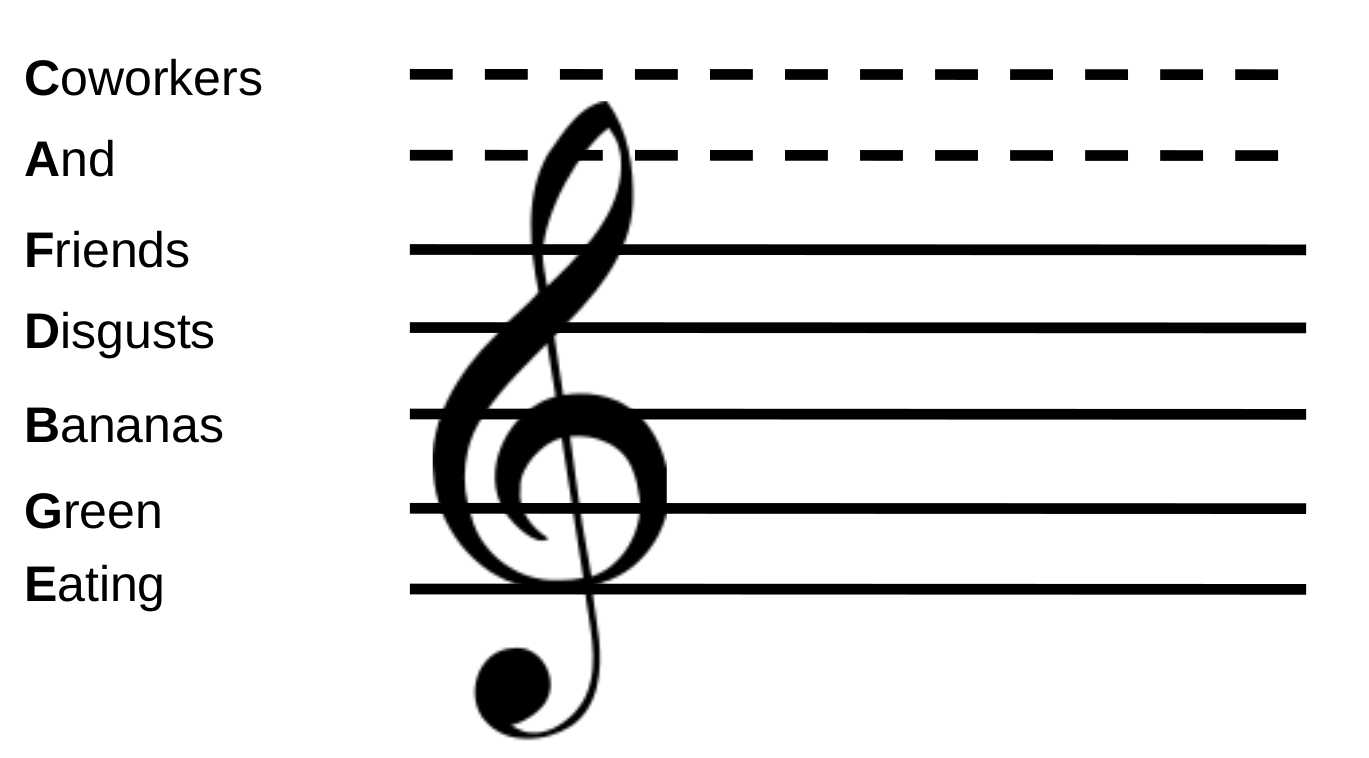
\includegraphics[width=8cm]{music-clef-mnemonic}
    };
    \draw[thick, ->] (0, -1.0) -- (10, -1.0) node[anchor=north east] {x (Time)};
    \draw[thick, ->] (0, -1.0) -- (0, 4.0) node[anchor=north east] {y (Frequency)};
  \end{tikzpicture}
  \label{fig:lilypond-music-clef-mnemonic}
  \caption{A mnemonic that helps to remember position of notes in the treble
    clef.}
\end{figure}

If we read the words from the bottom to the top, we get the humorous phrase
``\textbf{E}ating \textbf{G}reen \textbf{B}ananas \textbf{D}isgusts
\textbf{F}riends \textbf{A}nd \textbf{C}oworkers''.  The first letter encodes
the note in the scientific notation.  On the above we added two additional
dashed lines (aside from the five main ones).  The mnemonic encodes only the
notes on the lines, but with that we can figure out what notes are between the
lines as well.

\end{document}
